\documentclass[10pt,twocolumn,letterpaper]{article}

\usepackage{cvpr}
\usepackage{times}
\usepackage{epsfig}
\usepackage{graphicx}
\graphicspath{{./figures/}}
\usepackage{amsmath}
\usepackage{amssymb}

% Include other packages here, before hyperref.
\usepackage[breaklinks=true,bookmarks=false]{hyperref}

\cvprfinalcopy % *** Uncomment this line for the final submission

\begin{document}

%%%%%%%%% TITLE
\title{Layer-Wise Epistemic Ablation: Quantifying Structural Uncertainty \\ in Convolutional Neural Networks under Distribution Shift}

\author{Chen-Yi Su\\
Johns Hopkins University\\
{\tt\small csu@jhu.edu}
}

\maketitle

%%%%%%%%% ABSTRACT
\begin{abstract}
Convolutional networks are often overconfident under corruptions. We train a CIFAR-style ResNet-18 on CIFAR-10 with Monte Carlo (MC) dropout restricted to different layers: none, all blocks, only the first block, only the final fully connected layer, or the last block plus the head. On CIFAR-10-C, we report accuracy, Brier score, adaptive calibration error (ACE), and mutual information (MI) from $T{=}50$ forward passes. At the highest corruption severity, dropout in all blocks attains the lowest mean ACE among the stochastic modes we tried, while restricting dropout to the first block yields the highest mean accuracy but low MI, consistent with little epistemic disagreement at the output. The deterministic baseline shares the same Brier and ACE definitions but carries no MC-based MI. Code and checkpoints are organized in the accompanying project directory.
\end{abstract}

%%%%%%%%% 1. INTRODUCTION
\section{Introduction}

Deep learning classifiers deployed in real-world scenarios must not only be accurate but also provide reliable uncertainty estimates. However, modern convolutional neural networks are often overconfident, particularly when encountering corrupted inputs or out-of-distribution (OOD) data. Measuring this calibration degradation under distribution shift is challenging; traditional fixed-bin metrics like Expected Calibration Error (ECE) suffer from high statistical variance when predictive distributions skew heavily. To address this, Adaptive Calibration Error (ACE)~\cite{nixon2019measuring} was proposed, utilizing equal-frequency binning to stabilize the estimate.

To improve calibration and quantify uncertainty, Monte Carlo (MC) dropout~\cite{gal2016dropout} offers a computationally efficient ensemble approach by capturing epistemic uncertainty through predictive disagreement across forward passes~\cite{kendall2017what}. Yet, it is unclear which layers should remain stochastic if one desires both calibrated probabilities and stable feature representations. Recent studies advocate for restricting Bayesian approximations strictly to the final layer to preserve learned features and maintain efficiency~\cite{daxberger2021laplace,kristiadi2020being}, but their effectiveness under severe spatial corruptions remains an open question.

In this work, we conduct a controlled ablation study on a CIFAR-style ResNet-18 to investigate the spatial origin of epistemic uncertainty. Using a consistent training recipe, we evaluate five distinct placements of dropout during inference. We benchmark our models on CIFAR-10-C~\cite{hendrycks2019benchmarking} across five severity levels, reporting mean metrics over all corruption types. Section~\ref{sec:exp} presents the accuracy and ACE curves, while Section~\ref{sec:disc} interprets the stark contrast between early-block and full-network stochasticity, challenging the last-layer paradigm under extreme distribution shift.

%%%%%%%%% 2. THEORETICAL BACKGROUND & LITERATURE REVIEW
\section{Theoretical Background and Literature Review}

\subsection{Variational Inference and MC Dropout}
Standard deep neural networks (DNNs) yield deterministic point estimates, lacking the ability to express predictive uncertainty. To address this, Gal and Ghahramani \cite{gal2016dropout} demonstrated that applying Monte Carlo (MC) Dropout during inference is mathematically equivalent to performing approximate Bayesian variational inference. Specifically, it minimizes the Kullback-Leibler (KL) divergence between an approximate distribution $q(\omega)$ and the true posterior $p(\omega | X, Y)$. Building upon this foundation, Kendall and Gal \cite{kendall2017what} established an information-theoretic framework to disentangle total predictive entropy into two distinct components: aleatoric uncertainty (irreducible data noise) and epistemic uncertainty (reducible model ignorance). By calculating the Mutual Information (MI) between the predictions and the model posterior, we can isolate the epistemic component, which theoretically captures the model's structural doubt when encountering out-of-distribution (OOD) data.

\subsection{Calibration under Distribution Shift}
While modern DNNs achieve high in-distribution accuracy, they suffer from severe overconfidence \cite{guo2017calibration}. Traditionally, Expected Calibration Error (ECE) is used to measure the gap between model confidence and actual accuracy. However, ECE relies on fixed confidence binning, which introduces extreme statistical variance when predictive distributions shift heavily under OOD conditions. To resolve this, Nixon et al. \cite{nixon2019measuring} introduced the Adaptive Calibration Error (ACE), which utilizes adaptive binning to ensure an equal number of samples per bin, providing a statistically robust metric. To benchmark this calibration degradation realistically, Hendrycks and Dietterich \cite{hendrycks2019benchmarking} introduced CIFAR-10-C, a dataset of common corruptions, which Ovadia et al. \cite{ovadia2019can} subsequently established as the gold standard for stress-testing Bayesian uncertainty under dataset shift.

\subsection{Architecture and the Last-Layer Paradigm}
Implementing MC Dropout in modern CNN architectures requires careful structural consideration. Zagoruyko and Komodakis \cite{zagoruyko2016wide} demonstrated that the optimal placement for dropout within residual networks is strictly between the convolutional layers, preserving the identity mapping of the skip connections. More recently, the field of Bayesian Deep Learning has experienced a paradigm shift regarding where stochasticity should be applied. Kristiadi et al.~\cite{kristiadi2020being} showed that even approximate Bayesian inference such as applying uncertainty to a subset of parameters (e.g., the final layer) can mitigate overconfidence in ReLU networks. Daxberger et al.~\cite{daxberger2021laplace} demonstrated that restricting Bayesian inference to the final layer provides a strong trade-off between computational efficiency and predictive performance, often matching or outperforming full-network approximations in practice. Those claims motivate our ablation; Section~\ref{sec:disc} revisits them against CIFAR-10-C, where severe input corruptions may break the assumptions behind late-layer-only stochasticity.

%%%%%%%%% 3. METHODOLOGY
\section{Methodology}

\subsection{Model Architecture and Ablation Modes}
To prevent the aggressive downsampling inherent to ImageNet architectures, we utilize a customized CIFAR-ResNet-18 baseline. The standard $7 \times 7$ convolutional stem and max-pooling layers are replaced with a $3 \times 3$ convolution (stride 1) and an identity mapping, preserving the spatial resolution of the $32 \times 32$ CIFAR-10 inputs. 

To isolate the spatial origin of epistemic uncertainty, we define five architectural ablation modes. Spatial dropout (\texttt{Dropout2d}, $p=0.3$) is utilized \textbf{strictly between the two convolutional layers} within the residual blocks, while standard \texttt{Dropout} ($p=0.3$) is applied prior to the final fully connected (FC) layer:
\begin{itemize}
    \item \textbf{none:} A purely deterministic baseline with no stochasticity.
    \item \textbf{all:} Stochasticity applied across all residual blocks and the FC layer.
    \item \textbf{first\_block:} Spatial stochasticity restricted solely to the first residual block (early geometric features).
    \item \textbf{last\_layer\_strict:} All convolutional layers remain deterministic; stochasticity is injected solely at the final FC layer (semantic decision boundary).
    \item \textbf{last\_block\_plus\_fc:} Stochasticity applied to the final residual block and the FC layer.
\end{itemize}

\subsection{Inference Protocol and Variance Shift}
A critical challenge in evaluating MC Dropout is the variance shift induced by Batch Normalization (BN). If the model remains in full training mode during inference, BN aggregates batch-level statistics rather than utilizing the stable historical running means, artificially inflating aleatoric noise. To mitigate this, our inference protocol first sets the model to evaluation mode (freezing BN statistics), and subsequently iterates through the model modules to explicitly re-enable training mode exclusively for \texttt{Dropout} and \texttt{Dropout2d} layers. We perform $T=50$ stochastic forward passes per image for all Bayesian modes, and $T=1$ for the deterministic baseline.

\subsection{Uncertainty Quantification}
For each sample, we obtain $T$ softmax probability vectors, denoted as $\hat{p}^{(t)}$. The Bayesian average prediction is computed as $\bar{p} = \frac{1}{T}\sum_{t=1}^{T} \hat{p}^{(t)}$. We compute the Mutual Information (MI) to quantify epistemic uncertainty:
\begin{equation}
    MI = \mathcal{H}(\bar{p}) - \frac{1}{T}\sum_{t=1}^{T} \mathcal{H}(\hat{p}^{(t)})
\end{equation}
where $\mathcal{H}(\cdot)$ denotes the Shannon entropy. When $T{=}1$, the two terms coincide and MI is identically zero; we therefore interpret MI only for MC dropout modes with $T{=}50$. Brier score and ACE still use $\bar{p}$ and remain well defined for the deterministic baseline.

\subsection{Calibration Metrics}
Models are evaluated on the CIFAR-10-C OOD benchmark across 5 severity levels. We measure calibration using the Brier Score and Adaptive Calibration Error (ACE). The Brier Score is defined as $BS = \frac{1}{N} \sum_{i=1}^{N} \sum_{c=1}^{C} (\hat{p}_{ic} - y_{ic})^2$, where $y_{ic}$ is the one-hot encoded true label. For ACE, predictions are sorted by confidence and partitioned into $M=15$ equal-frequency bins. The ACE is defined as the unweighted mean of the absolute difference between accuracy and confidence across all bins, ensuring statistical robustness under extreme distribution shifts.

%%%%%%%%% 4. EXPERIMENTS
\section{Experimental Results}
\label{sec:exp}

\subsection{In-distribution validation accuracy}
Table~\ref{tab:clean-val} lists the validation accuracy at the epoch with lowest validation loss for each mode (same split as training). Differences between modes are modest; the larger gaps appear under corruption.

\begin{table}[t]
\centering
\caption{Best validation accuracy on clean CIFAR-10 (held-out fraction), at the epoch selected by minimum validation loss.}
\label{tab:clean-val}
\input{tables/clean_val_acc}
\end{table}

\subsection{CIFAR-10-C: mean accuracy and ACE}

\begin{figure*}[t]
\centering
\begin{minipage}[t]{0.48\textwidth}
\centering
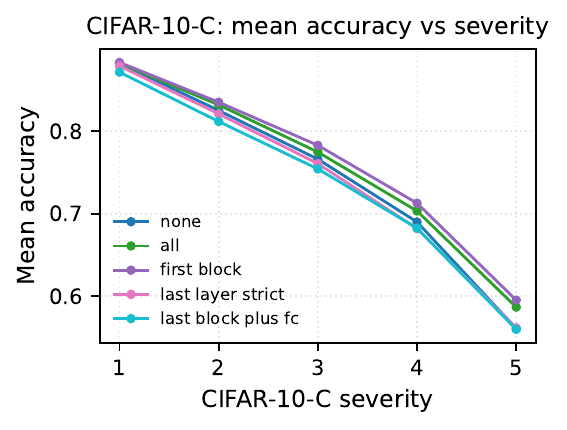
\includegraphics[width=\linewidth]{ood_mean_accuracy_severity.pdf}\\[-0.5ex]
{\footnotesize (a) Mean accuracy}
\end{minipage}\hfill
\begin{minipage}[t]{0.48\textwidth}
\centering
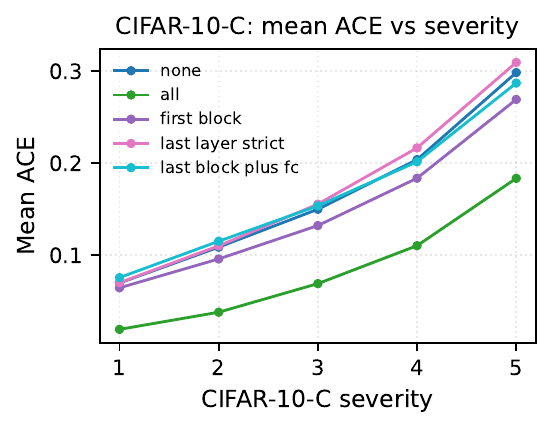
\includegraphics[width=\linewidth]{ood_mean_ace_severity.pdf}\\[-0.5ex]
{\footnotesize (b) Mean ACE}
\end{minipage}
\caption{CIFAR-10-C: metrics averaged over all benchmark corruptions. Lines denote dropout placement modes (see Section~3.1).}
\label{fig:ood-acc-ace}
\end{figure*}

\begin{figure}[t]
\centering
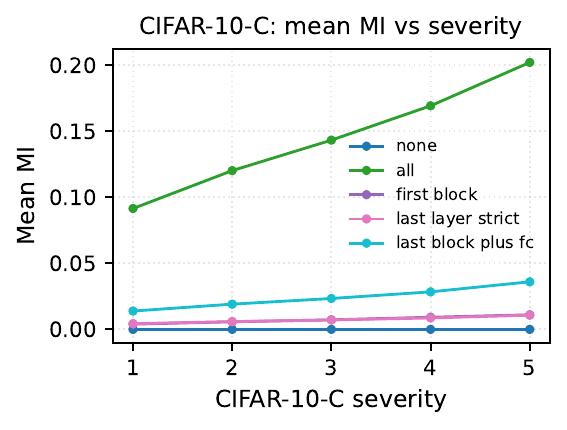
\includegraphics[width=\linewidth]{ood_mean_mi_severity.pdf}
\caption{Mean mutual information vs.\ severity (same averaging as Figure~\ref{fig:ood-acc-ace}). The \texttt{none} mode uses $T{=}1$; MI is not an epistemic signal there.}
\label{fig:ood-mi}
\end{figure}

Figure~\ref{fig:ood-acc-ace} averages accuracy and ACE over all corruptions in CIFAR-10-C for each severity. Accuracy falls as severity increases for every mode. Mean ACE generally rises with severity, reflecting growing miscalibration under stress.

Figure~\ref{fig:ood-mi} shows mean MI across corruptions. The deterministic baseline lies at zero by construction. Among stochastic modes, dropout in all blocks produces the largest MI at high severity, while restricting dropout to the first block keeps MI an order of magnitude smaller, indicating little spread in softmax outputs across passes despite non-trivial Brier and ACE.

\subsection{Snapshot at severity 5}
At severity 5, averaged over all benchmark corruptions in our run: mean accuracy was highest for \texttt{first\_block} ($\approx 0.60$); mean ACE was lowest for \texttt{all} ($\approx 0.18$); \texttt{last\_layer\_strict} reached the highest mean ACE among modes ($\approx 0.31$), slightly worse than the deterministic baseline \texttt{none} ($\approx 0.30$); mean MI was largest for \texttt{all} ($\approx 0.20$).

%%%%%%%%% 5. DISCUSSION
\section{Discussion}
\label{sec:disc}

\subsection{Early-block versus full-network dropout}
Early spatial dropout (\texttt{first\_block}) perturbs low-level features while the remaining trunk stays deterministic. The network produces comparatively accurate predictions, yet its MI stays small because the softmax outputs agree across all MC passes. This lack of epistemic disagreement indicates that the early-layer stochasticity fails to capture the model's actual miscalibration, which is evident from its non-trivial Brier and ACE scores. Full-network stochasticity (\texttt{all}) injects variation at every stage, which in our results tracks the largest MI at high severity and the lowest mean ACE at severity~5 among the modes we trained.

\subsection{Revisiting the last-layer paradigm under corruption}
Recent work advocates last-layer or late-layer Bayesian approximations as sufficient or preferable for calibration and efficiency~\cite{kristiadi2020being,daxberger2021laplace}. Our CIFAR-10-C results at severity~5 do not support that prescription under this experimental protocol.

As illustrated in Figure~\ref{fig:ood-acc-ace}, \texttt{last\_layer\_strict} exhibits the poorest calibration (ACE $\approx 0.31$), performing comparably to the deterministic baseline. By comparison, applying dropout across all blocks (\texttt{all}) achieves the lowest ACE ($\approx 0.18$) and the highest MI ($\approx 0.20$).

This discrepancy likely stems from how the models process severe spatial corruptions. In \texttt{last\_layer\_strict}, the deterministic convolutional trunk degrades early, passing corrupted features to the final layer. Perturbing this representation at the very end is insufficient to trigger meaningful epistemic disagreement. Full-network dropout avoids this bottleneck by allowing stochastic variations to accumulate throughout the network's hierarchy.

These results do not contradict the utility of last-layer approximations in the contexts originally proposed by those authors. Instead, they serve as an important boundary condition regarding severe covariate shift at the pixels. When the underlying feature extraction collapses entirely, late-layer uncertainty estimation becomes ineffective.


%%%%%%%%% 6. CONCLUSION
\section{Conclusion}

Layer placement for MC dropout changes both discrimination and uncertainty statistics on CIFAR-10-C. Full-network dropout increases epistemic MI under severe corruption and yields the lowest mean ACE among our modes at severity~5, whereas late-layer-only dropout matched or exceeded the deterministic baseline on mean ACE in our run. Early-only dropout keeps accuracy comparatively high but not epistemic spread at the softmax. The deterministic baseline supports Brier and ACE but not MC-based MI. Last-layer Bayesian approximations may still suit other OOD regimes; our evidence concerns pixel-level corruptions at high severity.

{\small
\bibliographystyle{ieee}
\bibliography{egbibfinal}
}

\end{document}